\documentclass[11pt,a4paper]{article}

% ---------- Fonts (premium: XCharter + Source Sans + Source Code Pro) ----------
\usepackage[T1]{fontenc}
\usepackage[utf8]{inputenc}
\usepackage[scaled=1.02]{XCharter}
\usepackage[semibold,scaled=0.94]{sourcesanspro}
\usepackage[scaled=0.82]{sourcecodepro}
\usepackage{textcomp}
\usepackage{amsmath}
\usepackage{microtype}

% ---------- Unicode passthrough so the source stays readable ----------
\usepackage{newunicodechar}
\newunicodechar{→}{\ensuremath{\rightarrow}}
\newunicodechar{←}{\ensuremath{\leftarrow}}
\newunicodechar{≤}{\ensuremath{\leq}}
\newunicodechar{≥}{\ensuremath{\geq}}
\newunicodechar{×}{\ensuremath{\times}}
\newunicodechar{−}{\textminus}
\newunicodechar{—}{\textemdash}
\newunicodechar{–}{\textendash}
\newunicodechar{“}{``}
\newunicodechar{”}{''}
\newunicodechar{‘}{`}
\newunicodechar{’}{'}
\newunicodechar{…}{\ldots}

% ---------- Layout ----------
\usepackage[a4paper,top=2.4cm,bottom=2.4cm,left=2.5cm,right=2.5cm]{geometry}
\usepackage{graphicx}
\usepackage{float}
\usepackage{enumitem}
\usepackage{booktabs}
\usepackage{tabularx}
\usepackage{array}
\usepackage{ragged2e}
\usepackage{colortbl}
\usepackage{caption}
\usepackage{titlesec}
\usepackage{fancyhdr}
\usepackage[section]{placeins}
\usepackage{xspace}
\usepackage[most]{tcolorbox}
\usepackage{tikz}
\usetikzlibrary{arrows.meta,positioning,calc,fit,backgrounds,shapes.geometric,
  decorations.pathreplacing,shadows.blur,shapes.multipart}

% ---------- Palette ----------
\definecolor{ink}{HTML}{1B2430}
\definecolor{inksoft}{HTML}{55606E}
\definecolor{accent}{HTML}{2F5C9E}   % blue  - read/used
\definecolor{green}{HTML}{3E8E5A}    % green - checked vs fixed value
\definecolor{amber}{HTML}{C08A1E}    % amber - files / capture
\definecolor{red}{HTML}{B03A3A}      % red   - attacker / deauth
\definecolor{gray}{HTML}{8A929C}     % gray  - present but unused
\definecolor{rule}{HTML}{2F5C9E}
\definecolor{pageband}{HTML}{EEF2F8}

\color{ink}
\linespread{1.06}

% ---------- Section styling ----------
\titleformat{\section}
  {\sffamily\bfseries\large\color{ink}}
  {\color{accent}\thesection\hspace{0.6em}}{0pt}
  {}[\vspace{2pt}{\color{rule}\titlerule[1pt]}]
\titleformat{\subsection}
  {\sffamily\bfseries\normalsize\color{accent!92!black}}
  {\thesubsection\hspace{0.5em}}{0pt}{}
\titleformat{\subsubsection}
  {\sffamily\bfseries\normalsize\color{ink}}
  {}{0pt}{}
\titlespacing*{\section}{0pt}{16pt}{7pt}
\titlespacing*{\subsection}{0pt}{11pt}{3pt}
\titlespacing*{\subsubsection}{0pt}{9pt}{2pt}

% ---------- Captions ----------
\captionsetup{font=small,labelfont={sf,bf,color=rule},textfont={sf},
  labelsep=period,skip=6pt,width=0.94\textwidth}

% ---------- Lists ----------
\setlist[itemize]{leftmargin=1.35em,itemsep=2.5pt,topsep=3pt,parsep=0pt}
\setlist[enumerate]{leftmargin=1.5em,itemsep=2.5pt,topsep=3pt}

% ---------- Tables ----------
\renewcommand{\arraystretch}{1.28}
\newcolumntype{L}[1]{>{\RaggedRight\arraybackslash}p{#1}}
\newcommand{\thd}[1]{\sffamily\bfseries\small\color{ink}#1}

% ---------- Header / footer ----------
\pagestyle{fancy}\fancyhf{}
\renewcommand{\headrulewidth}{0pt}
\fancyfoot[C]{\sffamily\footnotesize\color{inksoft}CSE406 — Topic 20 — WPA2 Handshake Capture, Offline Dictionary Attack \& WPA3-SAE Defense \;\textbullet\; Design Report}
\fancyfoot[R]{\sffamily\footnotesize\color{inksoft}\thepage}

% ---------- Inline helpers ----------
\newcommand{\code}[1]{{\ttfamily\small #1}}
\newcommand{\ra}{\ensuremath{\rightarrow}\xspace}
\usepackage{pifont}
\newcommand{\yes}{\textcolor{green}{\ding{51}}}
\newcommand{\dash}{\textcolor{gray}{\rule[0.35ex]{0.7em}{0.9pt}}}

% ---------- Console + callout boxes ----------
\newtcolorbox{console}{colback=ink!4,colframe=ink!22,boxrule=0.6pt,arc=2pt,
  left=8pt,right=8pt,top=5pt,bottom=5pt,fontupper=\ttfamily\scriptsize,
  before skip=6pt,after skip=6pt}
\newtcolorbox{whybox}{enhanced,colback=accent!5,colframe=accent!55,boxrule=0pt,
  leftrule=2.6pt,arc=1pt,left=10pt,right=10pt,top=7pt,bottom=7pt,
  before skip=8pt,after skip=8pt}

% ---------- Shared TikZ styles ----------
\tikzset{
  box/.style={draw,line width=0.8pt,rounded corners=3pt,align=center,inner sep=6pt},
  bRead/.style ={box,fill=accent!11,draw=accent!85!black,text=ink},
  bChk/.style  ={box,fill=green!14,draw=green!72!black,text=ink},
  bAmber/.style={box,fill=amber!16,draw=amber!85!black,text=ink},
  bRed/.style  ={box,fill=red!11,draw=red!78!black,text=ink},
  bOff/.style  ={box,fill=gray!16,draw=gray!85!black,text=ink},
  lbl/.style={font=\sffamily\scriptsize,text=inksoft,align=center},
  flow/.style={-{Stealth[length=3mm]},line width=1pt,draw=ink},
  flowred/.style={-{Stealth[length=2.6mm]},line width=1pt,draw=red!80!black,dashed},
  flowdot/.style={-{Stealth[length=2.6mm]},line width=1pt,draw=accent,densely dotted},
}

\usepackage[hidelinks,pdfusetitle]{hyperref}
\hypersetup{pdftitle={WPA2 Handshake Capture, Offline Dictionary Attack and WPA3-SAE Defense — Design Report},
  pdfauthor={CSE406 Topic 20 Group — 2105031, 2105057}}

% ============ editable group members ============
\newcommand{\groupmembers}{%
  \begin{tabular}{@{}L{6.9cm}@{}L{3.2cm}@{}}
    \thd{Name} & \thd{Student ID} \\[1pt]
    Nabiha Tahseen & \textcolor{inksoft}{2105031} \\
    Md.\ Mosharaf Hossain Apurbo & \textcolor{inksoft}{2105057} \\
  \end{tabular}}
\newcommand{\supervisorblock}{%
  {\sffamily\small\bfseries\color{ink}SUPERVISOR}\\[7pt]
  {\normalsize Imtiaz Kabir}\\[2pt]
  {\footnotesize\color{inksoft}Lecturer, Department of Computer Science and Engineering, BUET}}
% =================================================


% ---------- truth-table cell helpers ----------
\newcommand{\bit}[1]{{\sffamily\bfseries\color{accent}#1}}
\newcommand{\bz}{{\sffamily\color{gray}0}}
\newcommand{\dsh}{\textcolor{gray}{\textendash}}

% ---------- figure-specific TikZ styles ----------
\tikzset{
  % frame-layout (Fig 3)
  fR/.style={draw=accent!85!black,fill=accent!11,line width=0.8pt,rounded corners=2.5pt,minimum height=1.05cm,align=center,inner sep=2pt,font=\footnotesize,text=ink},
  fG/.style={draw=green!72!black,fill=green!15,line width=0.8pt,rounded corners=2.5pt,minimum height=1.05cm,align=center,inner sep=2pt,font=\footnotesize,text=ink},
  fO/.style={draw=gray!85!black,fill=gray!16,line width=0.8pt,rounded corners=2.5pt,minimum height=1.05cm,align=center,inner sep=2pt,font=\footnotesize,text=ink},
  ofl/.style={font=\sffamily\scriptsize,text=inksoft,align=center},
  sect/.style={font=\sffamily\bfseries\small,text=ink,anchor=south west},
  fn/.style={font=\ttfamily\scriptsize,text=accent!85!black},
  % bitfield (Fig 4)
  kR/.style={draw=accent!85!black,fill=accent!11,line width=0.8pt,rounded corners=2.5pt,minimum height=1.35cm,align=center,inner sep=2pt,font=\footnotesize,text=ink},
  kO/.style={draw=gray!85!black,fill=gray!16,line width=0.8pt,rounded corners=2.5pt,minimum height=1.35cm,align=center,inner sep=2pt,font=\footnotesize,text=ink},
  bitl/.style={font=\sffamily\scriptsize,text=inksoft},
  % flowchart (Fig 5)
  fclr/.style={draw,line width=0.9pt,rounded corners=3pt,align=center,inner sep=6pt,font=\small},
  cfg/.style ={fclr,fill=accent!7,draw=ink!55,text=ink},
  snif/.style={fclr,fill=amber!16,draw=amber!85!black,text=ink},
  deau/.style={fclr,fill=red!10,draw=red!75!black,text=ink},
  capf/.style={fclr,fill=amber!12,draw=amber!85!black,text=ink},
  hs/.style  ={fclr,fill=accent!11,draw=accent!85!black,text=ink},
  cr/.style  ={fclr,fill=green!13,draw=green!68!black,text=ink},
  cbox/.style={fclr,fill=green!15,draw=green!68!black,text=ink,font=\footnotesize,minimum height=1.25cm},
  term/.style={fclr,fill=gray!14,draw=gray!80!black,text=ink},
  dia/.style ={draw,line width=0.9pt,fill=amber!16,draw=amber!85!black,align=center,
               shape=diamond,aspect=2.2,inner sep=1pt,font=\small,text=ink},
  fg/.style={-{Stealth[length=2.6mm]},line width=1pt,draw=green!60!black},
}

% ================= FIGURE 1 : TOPOLOGY =================
\newcommand{\FIGONE}{%
\begin{figure}[!htb]\centering
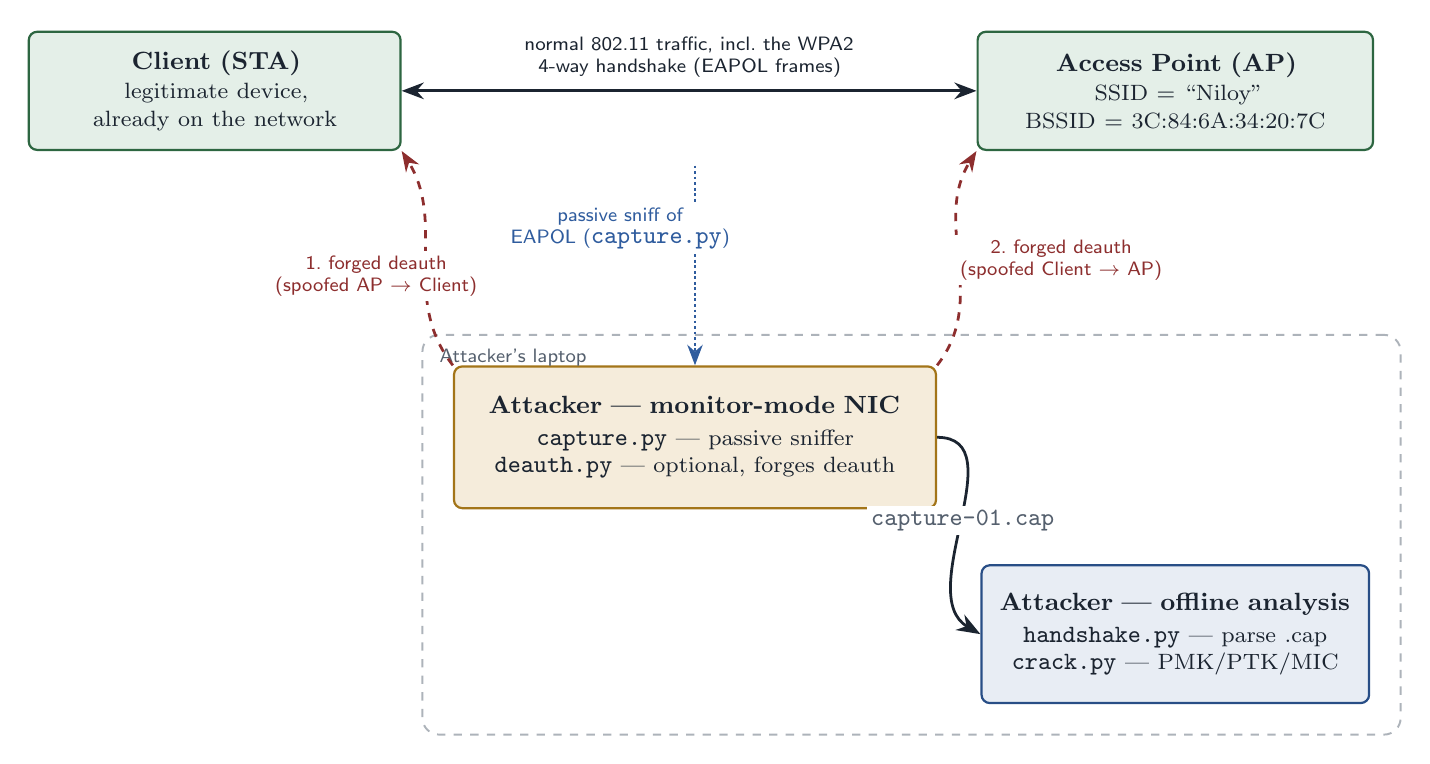
\begin{tikzpicture}[font=\small,node distance=0pt]
  \node[bChk,text width=4.3cm,minimum height=1.5cm] (client)
        at (0,4.7) {\textbf{Client (STA)}\\[1pt]\footnotesize legitimate device,\\[-1pt]\footnotesize already on the network};
  \node[bChk,text width=4.6cm,minimum height=1.5cm] (ap)
        at (12.2,4.7) {\textbf{Access Point (AP)}\\[1pt]\footnotesize SSID = ``Niloy''\\[-1pt]\footnotesize BSSID = 3C:84:6A:34:20:7C};
  \draw[{Stealth[length=2.8mm]}-{Stealth[length=2.8mm]},line width=1.1pt,draw=ink]
        (client.east) -- node[above,lbl,text=ink,yshift=1pt,align=center,text width=6.4cm]{normal 802.11 traffic, incl.\ the WPA2 4-way handshake (EAPOL frames)} (ap.west);
  \node[bAmber,text width=5.7cm,minimum height=1.8cm] (nic) at (6.1,0.3)
        {\textbf{Attacker --- monitor-mode NIC}\\[2pt]\footnotesize \code{capture.py} --- passive sniffer\\[-1pt]\footnotesize \code{deauth.py} --- optional, forges deauth};
  \node[bRead,text width=4.5cm,minimum height=1.75cm] (off) at (12.2,-2.2)
        {\textbf{Attacker --- offline analysis}\\[2pt]\footnotesize \code{handshake.py} --- parse .cap\\[-1pt]\footnotesize \code{crack.py} --- PMK/PTK/MIC};
  \begin{scope}[on background layer]
    \node[draw=gray!70,dashed,line width=0.7pt,rounded corners=6pt,
          fit=(nic)(off),inner sep=11pt] (lap) {};
  \end{scope}
  \node[lbl,anchor=north west,text=inksoft] at ([xshift=3pt,yshift=-2pt]lap.north west) {Attacker's laptop};
  \draw[flowdot] (6.1,3.75) -- (nic.north);
  \node[lbl,text=accent,fill=white,inner sep=1.8pt,align=center] at (5.15,2.95)
        {passive sniff of\\ EAPOL (\code{capture.py})};
  \draw[flowred] (nic.north west) to[out=128,in=-58] (client.south east);
  \node[lbl,text=red!80!black,fill=white,inner sep=1.8pt,align=center] at (2.05,2.35)
        {1.\ forged deauth\\ (spoofed AP $\rightarrow$ Client)};
  \draw[flowred] (nic.north east) to[out=52,in=-122] (ap.south west);
  \node[lbl,text=red!80!black,fill=white,inner sep=1.8pt,align=center] at (10.75,2.55)
        {2.\ forged deauth\\ (spoofed Client $\rightarrow$ AP)};
  \draw[flow] (nic.east) to[out=0,in=150] node[lbl,fill=white,inner sep=1.5pt,pos=0.5]{\code{capture-01.cap}} (off.west);
\end{tikzpicture}
\caption{Network topology. The attacker plays two separate roles: an on-air sniffer/injector and a purely offline analysis stage. Steps~1--2 (\code{deauth.py}) are optional --- sniffing and cracking still work if the client reconnects naturally, it just takes longer to wait for.}
\label{fig:topology}
\end{figure}}

% ================= FIGURE 2 : TIMING =================
\newcommand{\FIGTWO}{%
\begin{figure}[!htb]\centering
\resizebox{\textwidth}{!}{%
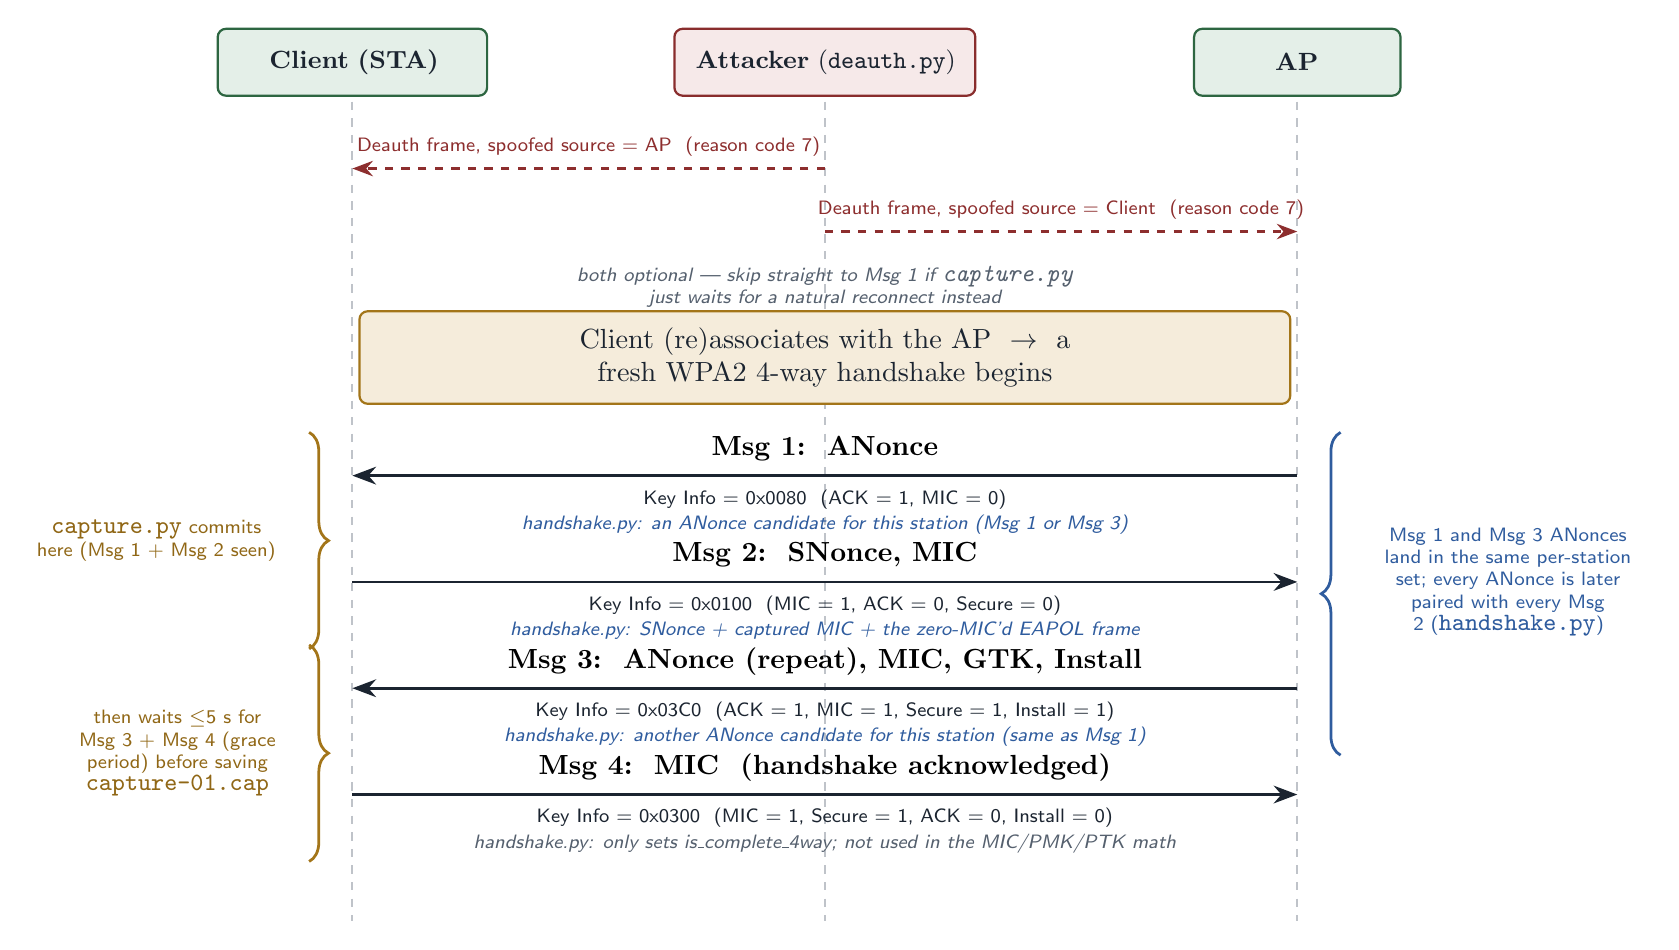
\begin{tikzpicture}[font=\small]
  \def\sta{0}\def\att{6}\def\ap{12}
  \def\ytop{0}\def\ybot{-10.9}
  \node[bChk,text width=3.0cm,minimum height=0.85cm] (hSTA) at (\sta,\ytop) {\textbf{Client (STA)}};
  \node[bRed,text width=3.4cm,minimum height=0.85cm] (hATT) at (\att,\ytop) {\textbf{Attacker} (\code{deauth.py})};
  \node[bChk,text width=2.2cm,minimum height=0.85cm] (hAP)  at (\ap,\ytop)  {\textbf{AP}};
  \foreach \x in {\sta,\att,\ap}
     \draw[gray!55,dashed,line width=0.7pt] (\x,-0.5) -- (\x,\ybot);
  \draw[flowred] (\att,-1.35) -- (\sta,-1.35);
  \node[lbl,text=red!80!black,above=0pt] at (\att/2+\sta/2,-1.32) {Deauth frame, spoofed source = AP\ \ (reason code 7)};
  \draw[flowred] (\att,-2.15) -- (\ap,-2.15);
  \node[lbl,text=red!80!black,above=0pt] at (\att/2+\ap/2,-2.12) {Deauth frame, spoofed source = Client\ \ (reason code 7)};
  \node[lbl,text=inksoft,align=center] at (\att,-2.85)
       {\itshape both optional --- skip straight to Msg 1 if \code{capture.py}\\ \itshape just waits for a natural reconnect instead};
  \node[bAmber,text width=11.4cm,minimum height=0.72cm,font=\normalsize] (reassoc) at (\att,-3.75)
       {Client (re)associates with the AP \ $\rightarrow$ \ a fresh WPA2 4-way handshake begins};
  \def\ma{-5.25}\def\mb{-6.60}\def\mc{-7.95}\def\md{-9.30}
  \node[font=\normalsize\bfseries] at (\att,\ma+0.34) {Msg 1:\ \ ANonce};
  \draw[flow] (\ap,\ma) -- (\sta,\ma);
  \node[lbl,text=ink] at (\att,\ma-0.30) {Key Info = 0x0080\ \ (ACK = 1, MIC = 0)};
  \node[lbl,text=accent,font=\sffamily\scriptsize\itshape] at (\att,\ma-0.62) {handshake.py: an ANonce candidate for this station (Msg 1 or Msg 3)};
  \node[font=\normalsize\bfseries] at (\att,\mb+0.34) {Msg 2:\ \ SNonce, MIC};
  \draw[flow] (\sta,\mb) -- (\ap,\mb);
  \node[lbl,text=ink] at (\att,\mb-0.30) {Key Info = 0x0100\ \ (MIC = 1, ACK = 0, Secure = 0)};
  \node[lbl,text=accent,font=\sffamily\scriptsize\itshape] at (\att,\mb-0.62) {handshake.py: SNonce + captured MIC + the zero-MIC'd EAPOL frame};
  \node[font=\normalsize\bfseries] at (\att,\mc+0.34) {Msg 3:\ \ ANonce (repeat), MIC, GTK, Install};
  \draw[flow] (\ap,\mc) -- (\sta,\mc);
  \node[lbl,text=ink] at (\att,\mc-0.30) {Key Info = 0x03C0\ \ (ACK = 1, MIC = 1, Secure = 1, Install = 1)};
  \node[lbl,text=accent,font=\sffamily\scriptsize\itshape] at (\att,\mc-0.62) {handshake.py: another ANonce candidate for this station (same as Msg 1)};
  \node[font=\normalsize\bfseries] at (\att,\md+0.34) {Msg 4:\ \ MIC\ \ (handshake acknowledged)};
  \draw[flow] (\sta,\md) -- (\ap,\md);
  \node[lbl,text=ink] at (\att,\md-0.30) {Key Info = 0x0300\ \ (MIC = 1, Secure = 1, ACK = 0, Install = 0)};
  \node[lbl,text=inksoft,font=\sffamily\scriptsize\itshape] at (\att,\md-0.62) {handshake.py: only sets is\_complete\_4way; not used in the MIC/PMK/PTK math};
  \draw[decorate,decoration={brace,amplitude=7pt},line width=1pt,amber!85!black]
       (\sta-0.55,\ma+0.55) -- (\sta-0.55,\mb-0.85);
  \node[lbl,text=amber!75!black,align=center,anchor=east] at (\sta-0.85,{(\ma+\mb)/2-0.15})
       {\code{capture.py} commits\\ here (Msg 1 + Msg 2 seen)};
  \draw[decorate,decoration={brace,amplitude=7pt},line width=1pt,amber!85!black]
       (\sta-0.55,\mc+0.55) -- (\sta-0.55,\md-0.85);
  \node[lbl,text=amber!75!black,align=center,anchor=east] at (\sta-0.85,{(\mc+\md)/2-0.15})
       {then waits $\leq$5 s for\\ Msg 3 + Msg 4 (grace\\ period) before saving\\ \code{capture-01.cap}};
  \draw[decorate,decoration={brace,mirror,amplitude=7pt},line width=1pt,accent]
       (\ap+0.55,\ma+0.55) -- (\ap+0.55,\mc-0.85);
  \node[lbl,text=accent,align=center,anchor=west,text width=3.4cm] at (\ap+0.85,{(\ma+\mc)/2})
       {Msg 1 and Msg 3 ANonces land in the same per-station set; every ANonce is later paired with every Msg 2 (\code{handshake.py})};
\end{tikzpicture}}
\caption{The WPA2 4-way handshake (the \emph{original protocol}, Msg 1--4) together with the attacker's optional \code{deauth.py} injection (the \emph{attack strategy}, top). Left braces mark exactly when \code{capture.py} commits and saves; the right brace shows how \code{handshake.py} pairs the captured nonces.}
\label{fig:timing}
\end{figure}}

% ================= FIGURE 3 : FRAME ENCAPSULATION =================
\newcommand{\FIGTHREE}{%
\begin{figure}[!htb]\centering
\resizebox{\textwidth}{!}{%
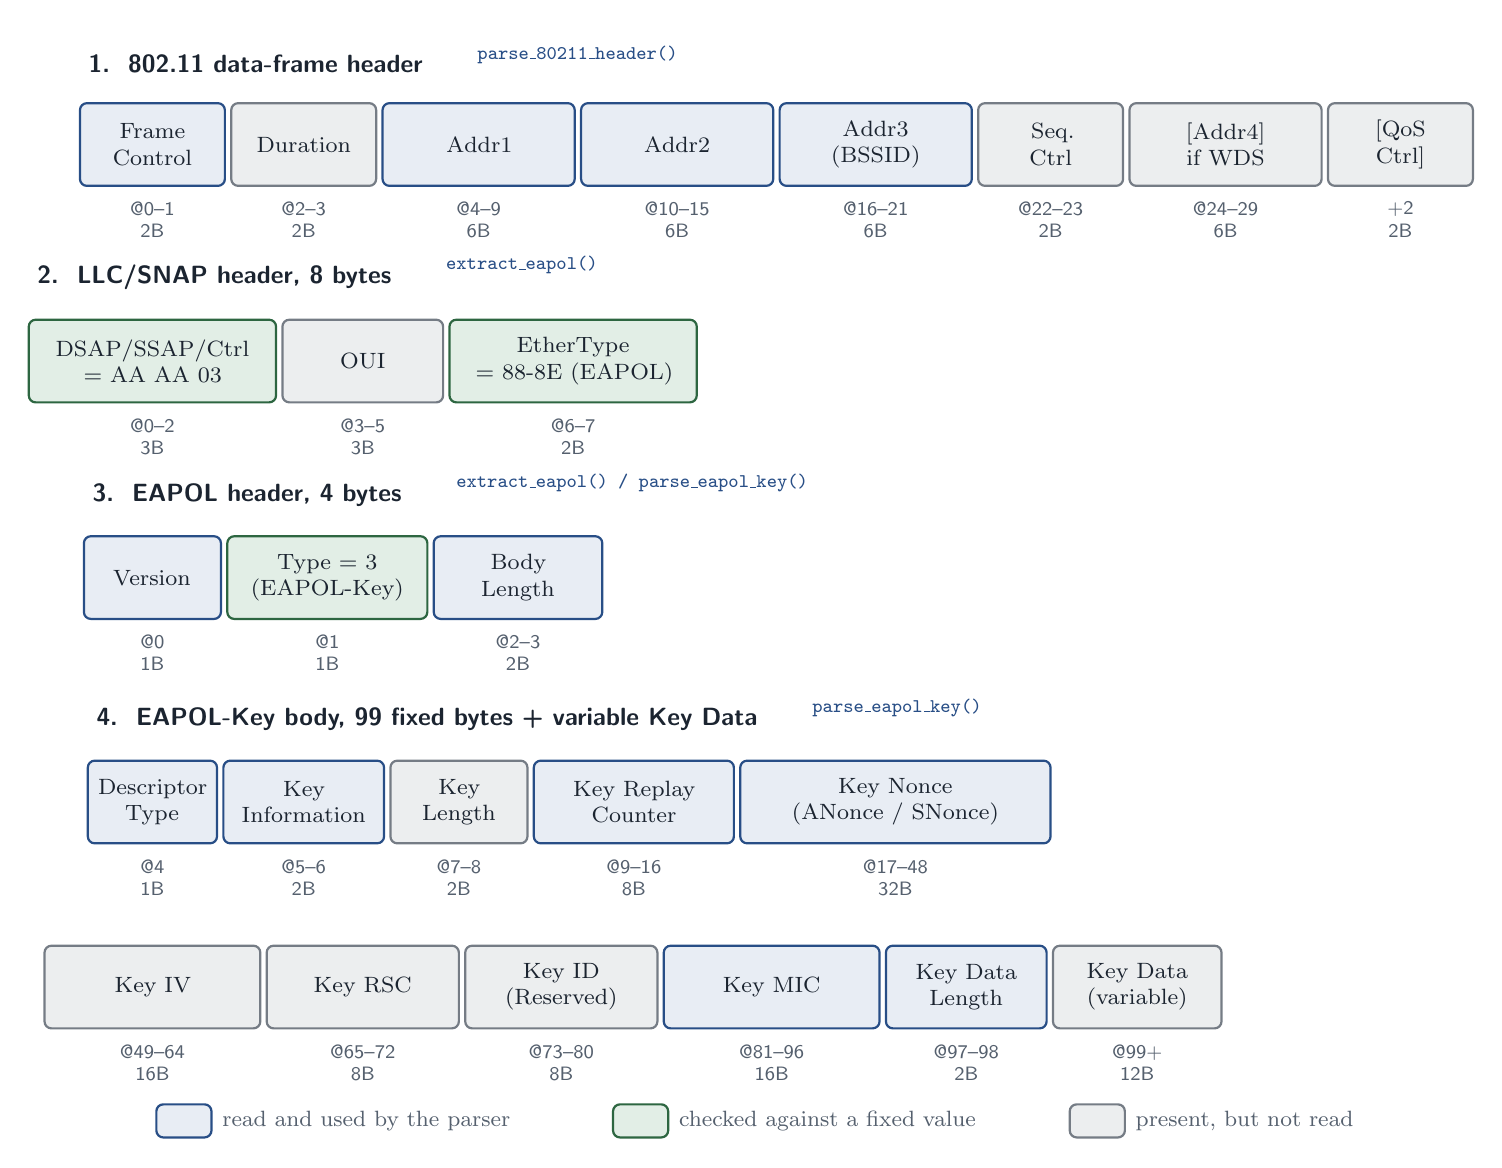
\begin{tikzpicture}
  \node[fR,text width=1.7cm] (a1) at (0,0) {Frame\\ Control};
  \node[fO,text width=1.7cm,right=1.5pt of a1] (a2) {Duration};
  \node[fR,text width=2.3cm,right=1.5pt of a2] (a3) {Addr1};
  \node[fR,text width=2.3cm,right=1.5pt of a3] (a4) {Addr2};
  \node[fR,text width=2.3cm,right=1.5pt of a4] (a5) {Addr3\\ (BSSID)};
  \node[fO,text width=1.7cm,right=1.5pt of a5] (a6) {Seq.\\ Ctrl};
  \node[fO,text width=2.3cm,right=1.5pt of a6] (a7) {[Addr4]\\ if WDS};
  \node[fO,text width=1.7cm,right=1.5pt of a7] (a8) {[QoS\\ Ctrl]};
  \node[ofl,below=2pt of a1]{@0--1\\2B};  \node[ofl,below=2pt of a2]{@2--3\\2B};
  \node[ofl,below=2pt of a3]{@4--9\\6B};  \node[ofl,below=2pt of a4]{@10--15\\6B};
  \node[ofl,below=2pt of a5]{@16--21\\6B};\node[ofl,below=2pt of a6]{@22--23\\2B};
  \node[ofl,below=2pt of a7]{@24--29\\6B};\node[ofl,below=2pt of a8]{+2\\2B};
  \node[sect] at ([yshift=7pt]a1.north west) {1.\ \ 802.11 data-frame header \ \ \ \ \tikz{\node[fn]{parse\_80211\_header()};}};
  \node[fG,text width=3.0cm] (b1) at (0,-2.75) {DSAP/SSAP/Ctrl\\ = AA AA 03};
  \node[fO,text width=1.9cm,right=1.5pt of b1] (b2) {OUI};
  \node[fG,text width=3.0cm,right=1.5pt of b2] (b3) {EtherType\\ = 88-8E (EAPOL)};
  \node[ofl,below=2pt of b1]{@0--2\\3B}; \node[ofl,below=2pt of b2]{@3--5\\3B}; \node[ofl,below=2pt of b3]{@6--7\\2B};
  \node[sect] at ([yshift=7pt]b1.north west) {2.\ \ LLC/SNAP header, 8 bytes \ \ \ \ \tikz{\node[fn]{extract\_eapol()};}};
  \node[fR,text width=1.6cm] (c1) at (0,-5.5) {Version};
  \node[fG,text width=2.4cm,right=1.5pt of c1] (c2) {Type = 3\\ (EAPOL-Key)};
  \node[fR,text width=2.0cm,right=1.5pt of c2] (c3) {Body\\ Length};
  \node[ofl,below=2pt of c1]{@0\\1B}; \node[ofl,below=2pt of c2]{@1\\1B}; \node[ofl,below=2pt of c3]{@2--3\\2B};
  \node[sect] at ([yshift=7pt]c1.north west) {3.\ \ EAPOL header, 4 bytes \ \ \ \ \tikz{\node[fn]{extract\_eapol() / parse\_eapol\_key()};}};
  \node[fR,text width=1.5cm] (d1) at (0,-8.35) {Descriptor\\ Type};
  \node[fR,text width=1.9cm,right=1.5pt of d1] (d2) {Key\\ Information};
  \node[fO,text width=1.6cm,right=1.5pt of d2] (d3) {Key\\ Length};
  \node[fR,text width=2.4cm,right=1.5pt of d3] (d4) {Key Replay\\ Counter};
  \node[fR,text width=3.8cm,right=1.5pt of d4] (d5) {Key Nonce\\ (ANonce / SNonce)};
  \node[ofl,below=2pt of d1]{@4\\1B}; \node[ofl,below=2pt of d2]{@5--6\\2B}; \node[ofl,below=2pt of d3]{@7--8\\2B};
  \node[ofl,below=2pt of d4]{@9--16\\8B}; \node[ofl,below=2pt of d5]{@17--48\\32B};
  \node[sect] at ([yshift=7pt]d1.north west) {4.\ \ EAPOL-Key body, 99 fixed bytes + variable Key Data \ \ \ \ \tikz{\node[fn]{parse\_eapol\_key()};}};
  \node[fO,text width=2.6cm] (e1) at (0,-10.7) {Key IV};
  \node[fO,text width=2.3cm,right=1.5pt of e1] (e2) {Key RSC};
  \node[fO,text width=2.3cm,right=1.5pt of e2] (e3) {Key ID\\ (Reserved)};
  \node[fR,text width=2.6cm,right=1.5pt of e3] (e4) {Key MIC};
  \node[fR,text width=1.9cm,right=1.5pt of e4] (e5) {Key Data\\ Length};
  \node[fO,text width=2.0cm,right=1.5pt of e5] (e6) {Key Data\\ (variable)};
  \node[ofl,below=2pt of e1]{@49--64\\16B}; \node[ofl,below=2pt of e2]{@65--72\\8B}; \node[ofl,below=2pt of e3]{@73--80\\8B};
  \node[ofl,below=2pt of e4]{@81--96\\16B}; \node[ofl,below=2pt of e5]{@97--98\\2B}; \node[ofl,below=2pt of e6]{@99+\\12B};
  \node[fR,minimum width=0.7cm,minimum height=0.42cm,text width=0.1cm] (lg1) at (0.4,-12.4) {};
  \node[anchor=west,font=\footnotesize,text=inksoft] at (lg1.east) {read and used by the parser};
  \node[fG,minimum width=0.7cm,minimum height=0.42cm,text width=0.1cm] (lg2) at (6.2,-12.4) {};
  \node[anchor=west,font=\footnotesize,text=inksoft] at (lg2.east) {checked against a fixed value};
  \node[fO,minimum width=0.7cm,minimum height=0.42cm,text width=0.1cm] (lg3) at (12.0,-12.4) {};
  \node[anchor=west,font=\footnotesize,text=inksoft] at (lg3.east) {present, but not read};
\end{tikzpicture}}
\caption{Frame encapsulation from the 802.11 header down to the EAPOL-Key body, with the exact byte offsets and field sizes used by the code. Offsets in layer~4 continue from byte~4 of the EAPOL frame.}
\label{fig:frame}
\end{figure}}

% ================= FIGURE 4 : KEY INFORMATION BITFIELD =================
\newcommand{\FIGFOUR}{%
\begin{figure}[!htb]\centering
\resizebox{\textwidth}{!}{%
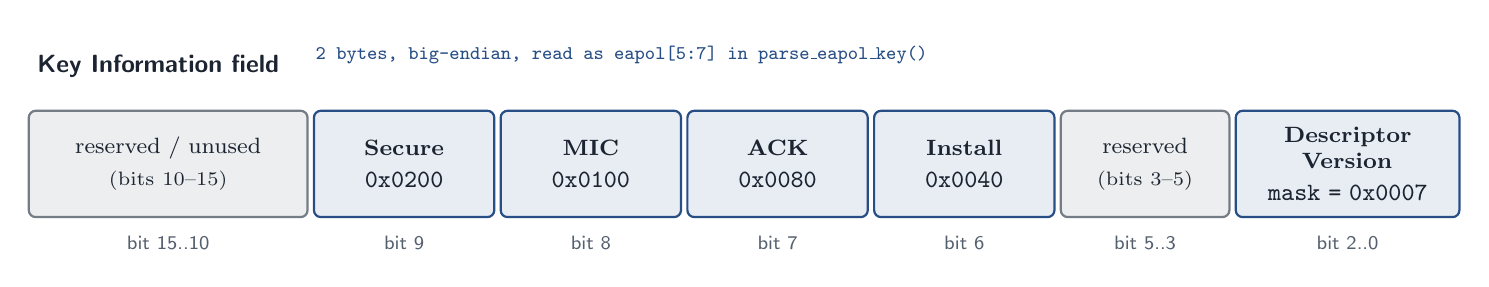
\begin{tikzpicture}
  \node[kO,text width=3.4cm] (k0) at (0,0) {reserved / unused\\[2pt]\scriptsize (bits 10--15)};
  \node[kR,text width=2.15cm,right=1.5pt of k0] (k1) {\textbf{Secure}\\[2pt]\code{0x0200}};
  \node[kR,text width=2.15cm,right=1.5pt of k1] (k2) {\textbf{MIC}\\[2pt]\code{0x0100}};
  \node[kR,text width=2.15cm,right=1.5pt of k2] (k3) {\textbf{ACK}\\[2pt]\code{0x0080}};
  \node[kR,text width=2.15cm,right=1.5pt of k3] (k4) {\textbf{Install}\\[2pt]\code{0x0040}};
  \node[kO,text width=2.0cm,right=1.5pt of k4] (k5) {reserved\\[2pt]\scriptsize (bits 3--5)};
  \node[kR,text width=2.7cm,right=1.5pt of k5] (k6) {\textbf{Descriptor Version}\\[2pt]\code{mask = 0x0007}};
  \foreach \n/\b in {k0/{bit 15..10},k1/{bit 9},k2/{bit 8},k3/{bit 7},k4/{bit 6},k5/{bit 5..3},k6/{bit 2..0}}
     \node[bitl,below=3pt of \n]{\b};
  \node[font=\sffamily\bfseries\small,text=ink,anchor=south west] at ([yshift=8pt]k0.north west)
     {Key Information field \ \ \tikz{\node[font=\ttfamily\scriptsize,text=accent!85!black]{2 bytes, big-endian, read as eapol[5:7] in parse\_eapol\_key()};}};
\end{tikzpicture}}
\caption{The Key Information bit field, decoded exactly as in \code{handshake.py}. \code{classify\_message()} names each message from these flags: \textbf{Msg 1} = ACK \& !MIC; \textbf{Msg 2} = MIC \& !ACK \& !Secure; \textbf{Msg 3} = ACK \& MIC \& Secure \& Install; \textbf{Msg 4} = MIC \& Secure \& !ACK \& !Install. Any other combination classifies as 0 and is ignored.}
\label{fig:keyinfo}
\end{figure}}

% ================= FIGURE 5 : PIPELINE FLOWCHART =================
\newcommand{\FIGFIVE}{%
\begin{figure}[!htb]\centering
\resizebox{0.99\textwidth}{!}{%
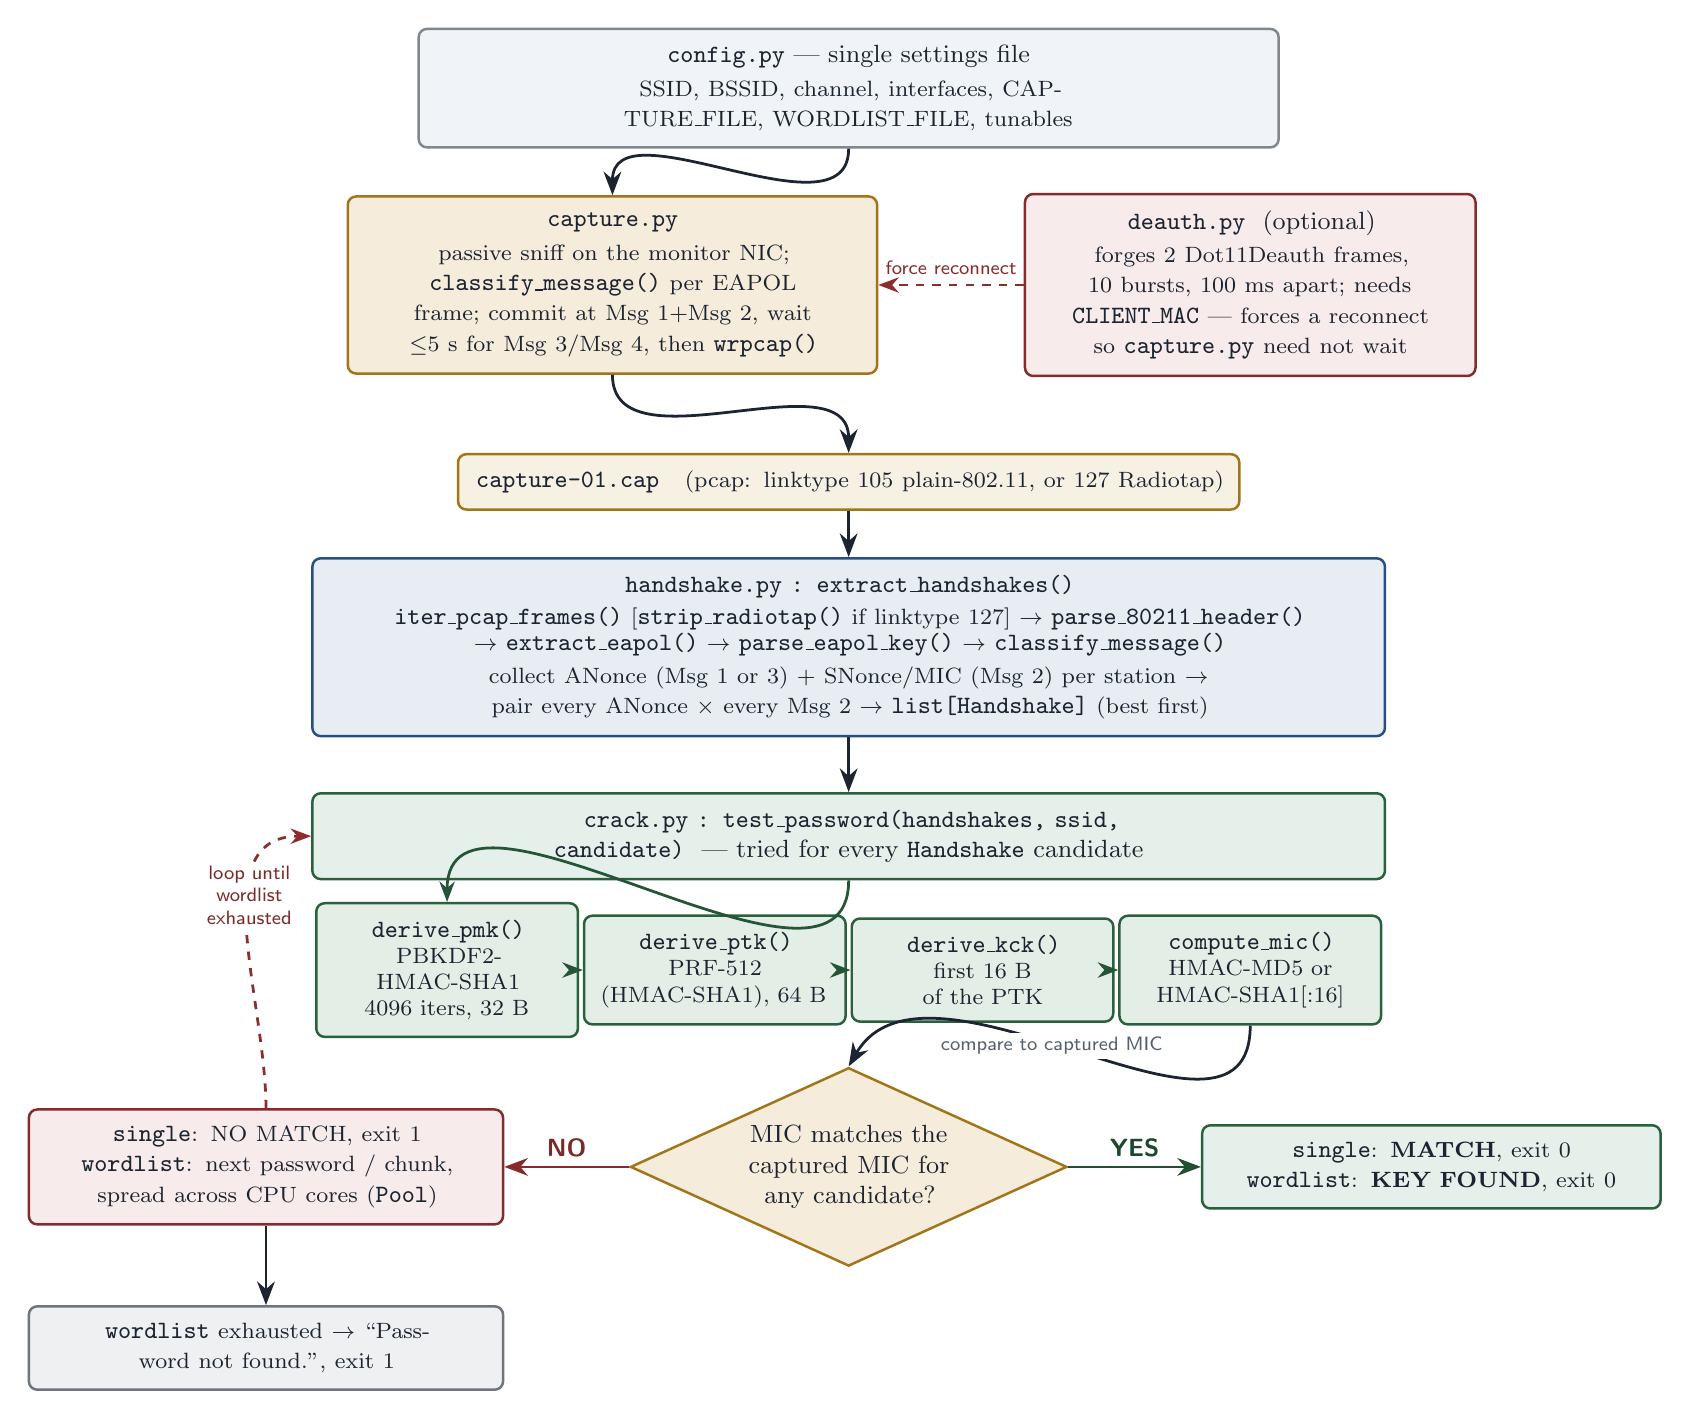
\begin{tikzpicture}
  \node[cfg,text width=10.5cm] (cfg) at (0,0)
     {\code{config.py} --- single settings file\\[1pt]\footnotesize SSID, BSSID, channel, interfaces, CAPTURE\_FILE, WORDLIST\_FILE, tunables};
  \node[snif,text width=6.3cm] (snif) at (-3.0,-2.5)
     {\code{capture.py}\\[1pt]\footnotesize passive sniff on the monitor NIC; \code{classify\_message()} per EAPOL frame; commit at Msg 1+Msg 2, wait $\leq$5 s for Msg 3/Msg 4, then \code{wrpcap()}};
  \node[deau,text width=5.3cm] (deau) at (5.1,-2.5)
     {\code{deauth.py} \ (optional)\\[1pt]\footnotesize forges 2 Dot11Deauth frames, 10 bursts, 100 ms apart; needs \code{CLIENT\_MAC} --- forces a reconnect so \code{capture.py} need not wait};
  \node[capf,text width=9.5cm] (capf) at (0,-5.0)
     {\code{capture-01.cap} \ \ \footnotesize(pcap: linktype 105 plain-802.11, or 127 Radiotap)};
  \node[hs,text width=13.2cm] (hs) at (0,-7.1)
     {\code{handshake.py : extract\_handshakes()}\\[2pt]\footnotesize \code{iter\_pcap\_frames()} [\code{strip\_radiotap()} if linktype 127] $\rightarrow$ \code{parse\_80211\_header()} $\rightarrow$ \code{extract\_eapol()} $\rightarrow$ \code{parse\_eapol\_key()} $\rightarrow$ \code{classify\_message()}\\[1pt]\footnotesize collect ANonce (Msg 1 or 3) + SNonce/MIC (Msg 2) per station $\rightarrow$ pair every ANonce $\times$ every Msg 2 $\rightarrow$ \code{list[Handshake]} (best first)};
  \node[cr,text width=13.2cm] (crk) at (0,-9.5)
     {\code{crack.py : test\_password(handshakes, ssid, candidate)} \ --- tried for every \code{Handshake} candidate};
  \node[cbox,text width=2.9cm] (c1) at (-5.1,-11.2){\code{derive\_pmk()}\\ PBKDF2-HMAC-SHA1\\ 4096 iters, 32 B};
  \node[cbox,text width=2.9cm] (c2) at (-1.7,-11.2){\code{derive\_ptk()}\\ PRF-512\\ (HMAC-SHA1), 64 B};
  \node[cbox,text width=2.9cm] (c3) at (1.7,-11.2){\code{derive\_kck()}\\ first 16 B\\ of the PTK};
  \node[cbox,text width=2.9cm] (c4) at (5.1,-11.2){\code{compute\_mic()}\\ HMAC-MD5 or\\ HMAC-SHA1[:16]};
  \node[dia,text width=3.0cm] (dia) at (0,-13.7){MIC matches the captured MIC for any candidate?};
  \node[cr,text width=5.4cm] (yes) at (7.4,-13.7)
     {\footnotesize\code{single}: \textbf{MATCH}, exit 0\\ \code{wordlist}: \textbf{KEY FOUND}, exit 0};
  \node[deau,text width=5.6cm] (no) at (-7.4,-13.7)
     {\footnotesize\code{single}: NO MATCH, exit 1\\ \code{wordlist}: next password / chunk, spread across CPU cores (\code{Pool})};
  \node[term,text width=5.6cm] (term) at (-7.4,-16.0)
     {\footnotesize\code{wordlist} exhausted $\rightarrow$ ``Password not found.'', exit 1};
  \draw[flow] (cfg.south) to[out=-90,in=90] (snif.north);
  \draw[flowred] (deau.west) -- node[lbl,above,text=red!75!black]{force reconnect} (snif.east);
  \draw[flow] (snif.south) to[out=-90,in=90] (capf.north);
  \draw[flow] (capf.south) -- (hs.north);
  \draw[flow] (hs.south) -- (crk.north);
  \draw[fg] (crk.south) to[out=-90,in=90] (c1.north);
  \draw[fg] (c1.east) -- (c2.west);
  \draw[fg] (c2.east) -- (c3.west);
  \draw[fg] (c3.east) -- (c4.west);
  \draw[flow] (c4.south) to[out=-90,in=60] node[lbl,text=inksoft,pos=0.55,fill=white,inner sep=1.5pt]{compare to captured MIC} (dia.north);
  \draw[flow,draw=green!55!black] (dia.east) -- node[lbl,above,text=green!50!black,font=\sffamily\bfseries\small]{YES} (yes.west);
  \draw[flow,draw=red!75!black] (dia.west) -- node[lbl,above,text=red!70!black,font=\sffamily\bfseries\small]{NO} (no.east);
  \draw[flow] (no.south) -- (term.north);
  \draw[flowred] (no.north) to[out=90,in=180]
        node[lbl,text=red!70!black,pos=0.62,fill=white,inner sep=1.5pt,align=center]{loop until\\ wordlist\\ exhausted} (crk.west);
\end{tikzpicture}}
\caption{The implementation pipeline, from \code{config.py} through to a \textsc{match} / \textsc{no match} decision. The four green boxes are the from-scratch crypto chain inside \code{test\_password()}; the dashed loop returns to \code{crack.py} for the next candidate until the wordlist is exhausted.}
\label{fig:pipeline}
\end{figure}}

% ================= FIGURE 6 : WHY THE OFFLINE ATTACK DIES UNDER SAE =================
\newcommand{\FIGSIX}{%
\begin{figure}[H]\centering
\resizebox{0.86\textwidth}{!}{%
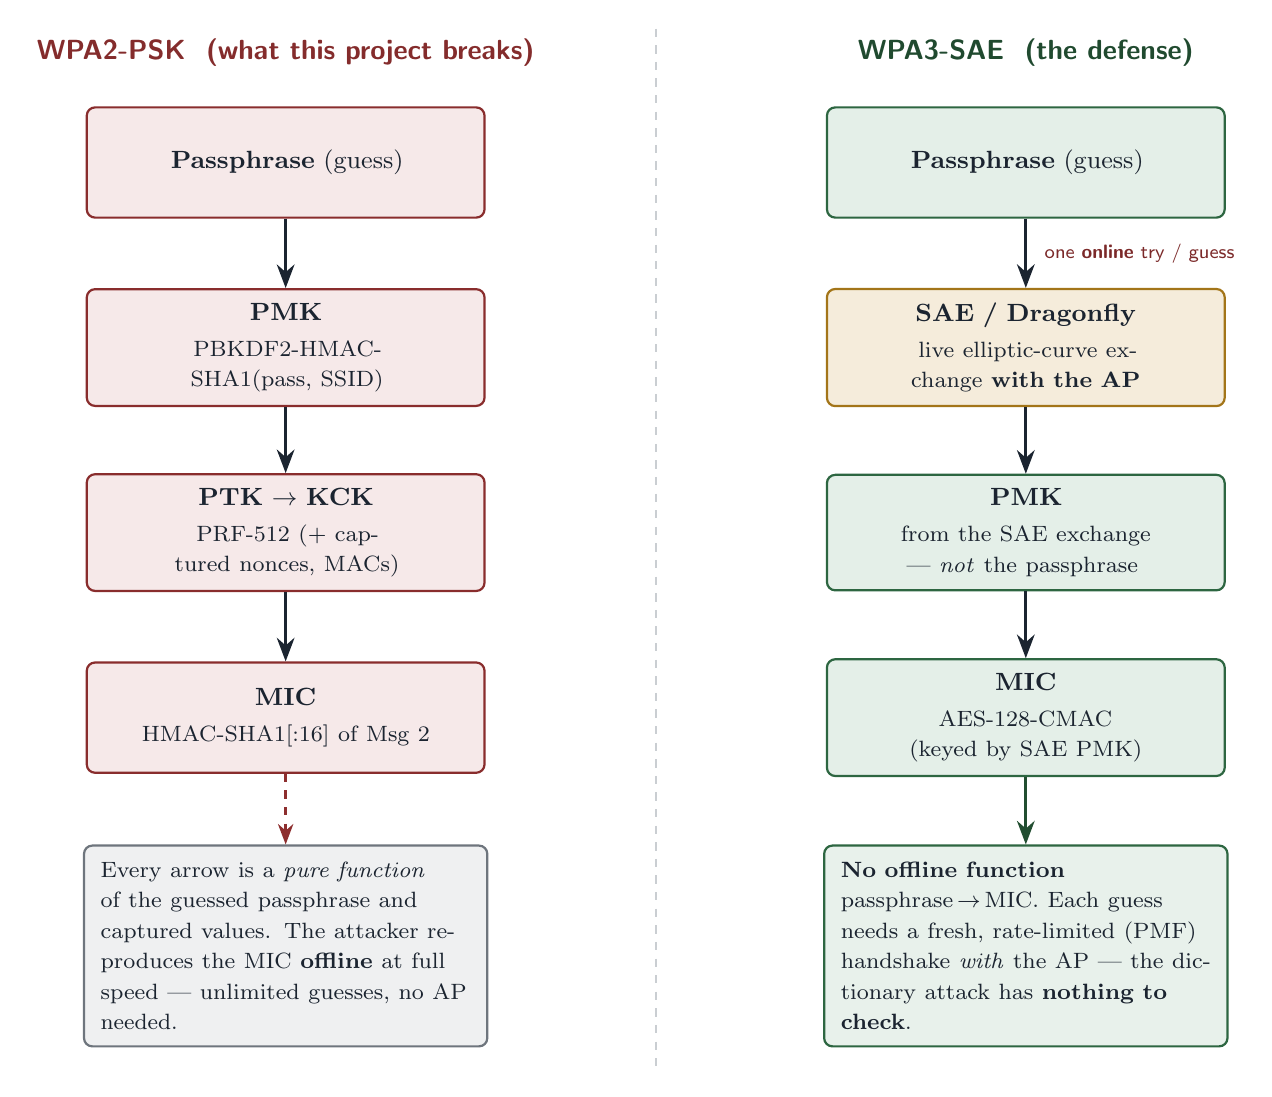
\begin{tikzpicture}[font=\small,node distance=0pt]
  \def\lx{-4.7}\def\rx{4.7}
  \def\ya{0}\def\yb{-2.35}\def\yc{-4.7}\def\yd{-7.05}
  \tikzset{chain/.style={rounded corners=3pt,align=center,inner sep=5pt,line width=0.8pt,
      text width=4.7cm,minimum height=1.4cm,text=ink},
    note/.style={rounded corners=3pt,align=left,inner sep=6pt,line width=0.8pt,
      text width=4.7cm,text=ink}}
  % --- column headers ---
  \node[font=\sffamily\bfseries,text=red!75!black] at (\lx,1.4) {WPA2-PSK\ \ (what this project breaks)};
  \node[font=\sffamily\bfseries,text=green!52!black] at (\rx,1.4) {WPA3-SAE\ \ (the defense)};
  % --- LEFT: WPA2 chain ---
  \node[chain,fill=red!11,draw=red!78!black] (lp) at (\lx,\ya) {\textbf{Passphrase} (guess)};
  \node[chain,fill=red!11,draw=red!78!black] (l1) at (\lx,\yb) {\textbf{PMK}\\[2pt]\footnotesize PBKDF2-HMAC-SHA1(pass, SSID)};
  \node[chain,fill=red!11,draw=red!78!black] (l2) at (\lx,\yc) {\textbf{PTK $\rightarrow$ KCK}\\[2pt]\footnotesize PRF-512 (+ captured nonces, MACs)};
  \node[chain,fill=red!11,draw=red!78!black] (l3) at (\lx,\yd) {\textbf{MIC}\\[2pt]\footnotesize HMAC-SHA1$[{:}16]$ of Msg 2};
  \draw[flow] (lp.south) -- (l1.north);
  \draw[flow] (l1.south) -- (l2.north);
  \draw[flow] (l2.south) -- (l3.north);
  \node[note,fill=gray!14,draw=gray!80!black] (lnote) at (\lx,-9.95)
     {\footnotesize Every arrow is a \emph{pure function} of the guessed passphrase and captured values. The attacker reproduces the MIC \textbf{offline} at full speed --- unlimited guesses, no AP needed.};
  \draw[flowred] (l3.south) -- (lnote.north);
  % --- RIGHT: WPA3 chain ---
  \node[chain,fill=green!14,draw=green!72!black] (rp) at (\rx,\ya) {\textbf{Passphrase} (guess)};
  \node[chain,fill=amber!16,draw=amber!85!black] (r1) at (\rx,\yb) {\textbf{SAE / Dragonfly}\\[2pt]\footnotesize live elliptic-curve exchange \textbf{with the AP}};
  \node[chain,fill=green!14,draw=green!72!black] (r2) at (\rx,\yc) {\textbf{PMK}\\[2pt]\footnotesize from the SAE exchange --- \emph{not} the passphrase};
  \node[chain,fill=green!14,draw=green!72!black] (r3) at (\rx,\yd) {\textbf{MIC}\\[2pt]\footnotesize AES-128-CMAC (keyed by SAE PMK)};
  \draw[flow] (rp.south) -- node[lbl,right=3pt,text=red!70!black]{one \textbf{online} try / guess} (r1.north);
  \draw[flow] (r1.south) -- (r2.north);
  \draw[flow] (r2.south) -- (r3.north);
  \node[note,fill=green!12,draw=green!72!black] (rnote) at (\rx,-9.95)
     {\footnotesize \textbf{No offline function} passphrase\,$\rightarrow$\,MIC. Each guess needs a fresh, rate-limited (PMF) handshake \emph{with} the AP --- the dictionary attack has \textbf{nothing to check}.};
  \draw[flow,draw=green!55!black] (r3.south) -- (rnote.north);
  % --- divider ---
  \draw[gray!45,line width=0.7pt,dashed] (0,1.7) -- (0,-11.5);
\end{tikzpicture}}
\caption{The same offline attack, side by side, against WPA2-PSK and WPA3-SAE. In WPA2 the whole PMK\,$\rightarrow$\,PTK\,$\rightarrow$\,MIC chain is a deterministic function of the guessed passphrase, so it can be replayed offline (left). In WPA3-SAE the PMK is produced by a \emph{live} elliptic-curve exchange with the AP, so no captured transcript lets an attacker turn a passphrase guess into the captured MIC (right) --- the vulnerability is removed at the root, not merely hidden.}
\label{fig:sae}
\end{figure}}

% ================= FIGURE 7 : SAE + PMF TIMING =================
\newcommand{\FIGSEVEN}{%
\begin{figure}[H]\centering
\resizebox{0.95\textwidth}{!}{%
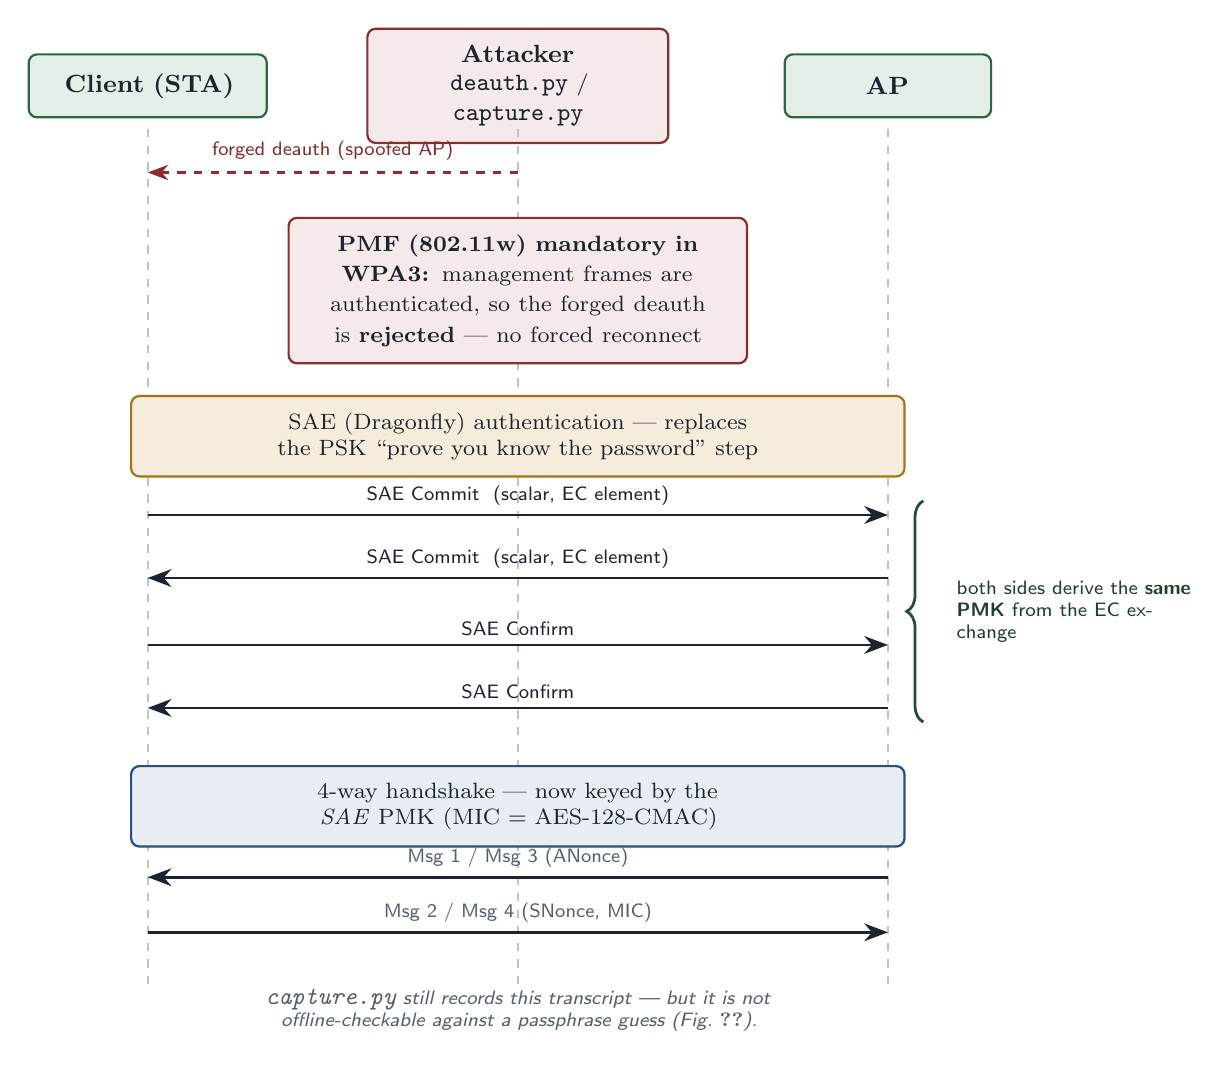
\begin{tikzpicture}[font=\small]
  \def\sta{0}\def\att{4.7}\def\ap{9.4}
  \def\ybot{-11.5}
  \node[bChk,text width=2.6cm,minimum height=0.8cm] (hSTA) at (\sta,0) {\textbf{Client (STA)}};
  \node[bRed,text width=3.4cm,minimum height=0.8cm] (hATT) at (\att,0) {\textbf{Attacker}\\[-1pt]\footnotesize \code{deauth.py} / \code{capture.py}};
  \node[bChk,text width=2.2cm,minimum height=0.8cm] (hAP)  at (\ap,0)  {\textbf{AP}};
  \foreach \x in {\sta,\att,\ap} \draw[gray!55,dashed,line width=0.7pt] (\x,-0.55) -- (\x,\ybot);
  % --- forged deauth blocked by PMF ---
  \draw[flowred] (\att,-1.1) -- (\sta,-1.1);
  \node[lbl,text=red!75!black,above=0pt] at ({(\att+\sta)/2},-1.07) {forged deauth (spoofed AP)};
  \node[bRed,text width=5.4cm,align=center] at (\att,-2.6)
     {\footnotesize \textbf{PMF (802.11w) mandatory in WPA3:} management frames are authenticated, so the forged deauth is \textbf{rejected} --- no forced reconnect};
  % --- SAE section ---
  \node[bAmber,text width=9.4cm,minimum height=0.55cm,font=\footnotesize] (sae) at ({(\sta+\ap)/2},-4.45)
     {SAE (Dragonfly) authentication --- replaces the PSK ``prove you know the password'' step};
  \def\ca{-5.45}\def\cb{-6.25}\def\cc{-7.1}\def\cd{-7.9}
  \draw[flow] (\sta,\ca) -- (\ap,\ca);
  \node[lbl,text=ink,above=0pt] at ({(\sta+\ap)/2},\ca) {SAE Commit\ \ (scalar, EC element)};
  \draw[flow] (\ap,\cb) -- (\sta,\cb);
  \node[lbl,text=ink,above=0pt] at ({(\sta+\ap)/2},\cb) {SAE Commit\ \ (scalar, EC element)};
  \draw[flow] (\sta,\cc) -- (\ap,\cc);
  \node[lbl,text=ink,above=0pt] at ({(\sta+\ap)/2},\cc) {SAE Confirm};
  \draw[flow] (\ap,\cd) -- (\sta,\cd);
  \node[lbl,text=ink,above=0pt] at ({(\sta+\ap)/2},\cd) {SAE Confirm};
  \draw[decorate,decoration={brace,mirror,amplitude=6pt},line width=1pt,green!55!black]
       (\ap+0.45,\ca+0.18) -- (\ap+0.45,\cd-0.18);
  \node[lbl,text=green!45!black,align=left,anchor=west,text width=3.0cm] at (\ap+0.75,{(\ca+\cd)/2})
       {both sides derive the \textbf{same PMK} from the EC exchange};
  % --- 4-way handshake keyed by SAE PMK ---
  \node[bRead,text width=9.4cm,minimum height=0.5cm,font=\footnotesize] (fw) at ({(\sta+\ap)/2},-9.15)
     {4-way handshake --- now keyed by the \emph{SAE} PMK (MIC = AES-128-CMAC)};
  \draw[flow] (\ap,-10.05) -- (\sta,-10.05);
  \node[lbl,above=0pt] at ({(\sta+\ap)/2},-10.05) {Msg 1 / Msg 3 (ANonce)};
  \draw[flow] (\sta,-10.75) -- (\ap,-10.75);
  \node[lbl,above=0pt] at ({(\sta+\ap)/2},-10.75) {Msg 2 / Msg 4 (SNonce, MIC)};
  \node[lbl,text=inksoft,align=center,anchor=north,text width=10.5cm] at ({(\sta+\ap)/2},-11.35)
     {\itshape \code{capture.py} still records this transcript --- but it is not offline-checkable against a passphrase guess (Fig.~\ref{fig:sae}).};
\end{tikzpicture}}
\caption{WPA3-SAE with mandatory PMF. The forged deauthentication frame \code{deauth.py} relies on is rejected as unauthenticated (top). Authentication is then done by the SAE Commit/Confirm exchange, whose PMK comes from live elliptic-curve material; the subsequent 4-way handshake is keyed by that PMK, so the captured handshake carries nothing an offline dictionary attack can test.}
\label{fig:saetiming}
\end{figure}}


\begin{document}
\thispagestyle{empty}

% ---------------- TITLE PAGE ----------------
\begin{center}
\vspace*{1.4cm}
{\color{rule}\rule{\textwidth}{1.4pt}}\\[4pt]
{\sffamily\footnotesize\color{inksoft}%
 \MakeUppercase{\hspace{0.15em}C\,S\,E\,4\,0\,6 \ \textbullet\ \ Security Sessional \ \textbullet\ \ Design Report}}\\[6pt]
{\color{rule}\rule{\textwidth}{0.6pt}}

\vspace{2.2cm}
{\sffamily\color{accent}\large Topic 20 --- Wi-Fi Password Cracking Attack \& Defense}\\[1.0cm]
{\bfseries\fontsize{27}{31}\selectfont WPA2 Handshake Capture,}\\[4pt]
{\bfseries\fontsize{27}{31}\selectfont Offline Dictionary Attack}\\[4pt]
{\bfseries\fontsize{27}{31}\selectfont \& WPA3-SAE Defense}\\[0.9cm]
{\large\itshape\color{inksoft} A from-scratch WPA2-PSK attack --- our own EAPOL parsing\\[2pt]
 and PMK/PTK/MIC cryptography --- with a working WPA3-SAE defense demonstration.}\\[10pt]
\begin{minipage}{0.82\textwidth}\centering\small\color{inksoft}
No \code{aircrack-ng}, \code{hashcat}, \code{pyrit} or \code{hcxtools}. \code{scapy} is used only to
sniff and craft raw 802.11 frames --- never for the cracking mathematics.
\end{minipage}

\vspace{2.4cm}
{\color{rule}\rule{0.5\textwidth}{0.6pt}}\\[10pt]
{\sffamily\small\bfseries\color{ink}GROUP MEMBERS}\\[8pt]
\groupmembers

\vspace{1.0cm}
\supervisorblock

\vfill
{\sffamily\footnotesize\color{inksoft}Department of Computer Science and Engineering, BUET \\[2pt]
Design Report --- submitted for evaluation}
\end{center}
\clearpage

% ============================================================
\section{Overview of the Project Idea}

Most home and small-office Wi-Fi networks use WPA2-PSK security: every device that joins types in the same shared password (the ``Wi-Fi password''). That password is never sent over the air. Instead, when a device connects, it and the access point (AP) run a short exchange called the \textbf{4-way handshake} to prove to each other that they both know the password, without either one ever transmitting it in the clear. This handshake is carried inside a Wi-Fi management protocol called \textbf{EAPOL} (Extensible Authentication Protocol over LAN).

This project attacks that scheme end to end. It does \emph{not} try to guess the password by talking to the AP directly --- that would be slow and would get noticed. Instead, it \textbf{captures one handshake off the air}, and then, completely \textbf{offline}, tries candidate passwords from a wordlist until one of them reproduces the exact cryptographic proof seen in the captured handshake. This is possible because the handshake contains enough information for anyone holding a candidate password to check, by themselves, whether that password is the right one --- the AP does not need to be asked.

\subsection{Two phases}
The project is split into an \textbf{online phase} (needs a wireless card in radio range of the target) and an \textbf{offline phase} (needs only the saved capture file, and can run anywhere, later, on any machine):

\begin{itemize}
\item \textbf{Online} --- \code{capture.py} passively listens for a client completing the 4-way handshake with the target AP and saves it to a file. \code{deauth.py} is an optional accelerant: it forges Wi-Fi deauthentication frames to knock a connected client offline so it reconnects immediately, instead of waiting for that to happen naturally.
\item \textbf{Offline} --- \code{handshake.py} parses the saved capture file into candidate handshakes, and \code{crack.py} runs the actual dictionary attack: for each candidate password, it derives the same keys the AP and client would have derived, and checks whether they match what was captured.
\end{itemize}

\subsection{What is, and is not, reused}
The cracking mathematics --- pcap parsing, 802.11/EAPOL frame decoding, PMK/PTK derivation, and MIC verification, in \code{handshake.py} and \code{crack.py} --- is a from-scratch implementation with \textbf{zero third-party cracking dependencies}: no \code{aircrack-ng}, \code{hashcat}, \code{pyrit}, or \code{hcxtools} is invoked anywhere. \code{capture.py} and \code{deauth.py} use the \code{scapy} library for one job only --- sniffing and crafting raw 802.11 radio frames --- in place of tools like \code{airodump-ng}/\code{aireplay-ng}. This distinction matters for the rest of the report: sections~\ref{sec:frame}--\ref{sec:justify} describe code that this project wrote and controls, not the behaviour of an external tool.

\subsection{Scope}
The target is \textbf{WPA2-PSK} (personal / pre-shared-key) networks specifically, using CCMP (AES) or TKIP pairwise ciphers --- the common case for home routers. Enterprise Wi-Fi (802.1X with a RADIUS server, a different key hierarchy) is out of scope. WPA3-SAE is out of scope as an \emph{attack} target --- and is in fact the centrepiece of our \emph{defense} (section~\ref{sec:defense}), which we both design and demonstrate in code.

\subsection{Division of work}
The two phases split cleanly along the online/offline boundary, and the work was divided the same way; both members jointly integrated, tested, and wrote the report.

\begin{table}[H]\centering\small
\setlength{\tabcolsep}{9pt}
\begin{tabularx}{\textwidth}{@{}L{4.9cm} L{9.2cm}@{}}
\toprule
\thd{Member} & \thd{Responsible for} \\
\midrule
Nabiha Tahseen \newline (2105031) & \textbf{Online phase} --- \code{capture.py} and \code{deauth.py}: monitor-mode setup, passive EAPOL sniffing, and from-scratch 802.11 deauthentication-frame crafting/injection with \code{scapy}; live capture during the demo. \\
Md.\ Mosharaf Hossain Apurbo \newline (2105057) & \textbf{Offline phase and defense} --- \code{handshake.py} (pcap/802.11/EAPOL parser), \code{crack.py} (PMK/PTK/MIC cryptography and the wordlist engine), \code{test\_crack.py}, and the WPA3-SAE defense (\code{wpa3\_demo.py}). \\
\midrule
Both members & \code{config.py}, end-to-end integration and testing, and this report. \\
\bottomrule
\end{tabularx}
\caption{Division of work between the two group members.}
\end{table}

% ============================================================
\section{Network Topology, Components and Timing}

Three parties are involved: a legitimate \textbf{Client (STA)} that already has the Wi-Fi password and is on the network; the target \textbf{Access Point (AP)}, identified by a fixed hardware address called its BSSID; and the \textbf{Attacker}, who only needs a wireless network card capable of \emph{monitor mode} within radio range of both --- no prior access to the network is required. Monitor mode lets a wireless card read every frame it can physically hear on a channel, not just frames addressed to it, which is what makes passive sniffing possible.

\bigskip
\FIGONE

\subsection{Components}
The attack is five small scripts plus a settings file, with a sixth standalone script (\code{wpa3\_demo.py}) for the defense (section~\ref{sec:defense}). Each has a single, sharply-defined job, and the two offline scripts touch no radio at all.

\begin{table}[H]\centering\small
\setlength{\tabcolsep}{9pt}
\begin{tabularx}{\textwidth}{@{}>{\ttfamily}l L{5.3cm} L{5.3cm}@{}}
\toprule
\thd{File} & \thd{Role} & \thd{Notes} \\
\midrule
config.py & Single settings file: SSID, BSSID, channel, interfaces, file paths, tunables. & The only file meant to be edited by hand. \\
capture.py & Passively sniffs the monitor interface and saves a usable handshake. & Needs \code{scapy} and root. Never sends deauth frames itself. \\
deauth.py & Optional: forges deauth frames to force a client to reconnect. & Needs \code{scapy}, root, and \code{config.CLIENT\_MAC} set. \\
handshake.py & Parses the \code{.cap} file into candidate 4-way handshakes. & Pure standard library. No radio access needed. \\
crack.py & PMK/PTK/MIC crypto plus the \code{info} / \code{single} / \code{wordlist} CLI. & Pure standard library. No radio access needed. \\
test\_crack.py & Automated regression tests for the parser and crypto. & Runs against a real, saved capture file. \\
wpa3\_demo.py & \textbf{Defense demo:} reruns the exact offline attack against a WPA3-SAE capture and shows it fails. & Standalone; imports the others read-only. See section~\ref{sec:defense}. \\
\bottomrule
\end{tabularx}
\caption{The attack scripts and the settings file, plus the WPA3-SAE defense demo, with each one's single responsibility.}
\end{table}

\subsection{The 4-way handshake and its timing}
Once a client is connected, the AP and the client run four EAPOL messages back and forth to derive a fresh session key from the shared password without ever transmitting it. Each message carries a \emph{Key Information} field whose bits identify which of the four messages it is (see section~\ref{sec:keyinfo}). Figure~\ref{fig:timing} shows the original protocol together with the optional forged-deauth step, and marks exactly what each piece of code keeps or uses.

\FIGTWO

\begin{itemize}
\item \textbf{Msg 1} (AP\,$\rightarrow$\,Client): the AP sends a fresh random number, the \textbf{ANonce}.
\item \textbf{Msg 2} (Client\,$\rightarrow$\,AP): the client replies with its own random number, the \textbf{SNonce}, plus a \textbf{Message Integrity Code (MIC)} that only someone who derived the right session key could produce.
\item \textbf{Msg 3} (AP\,$\rightarrow$\,Client): the AP confirms and repeats the same ANonce, together with the group key and its own MIC.
\item \textbf{Msg 4} (Client\,$\rightarrow$\,AP): the client acknowledges. The handshake is now complete.
\end{itemize}

\code{capture.py} commits to a client as soon as it has seen that client's Msg 1 and Msg 2 --- that pair alone is enough to attack offline --- then waits up to \code{GRACE\_PERIOD\_SEC = 5} more seconds for a confirming Msg 3 and Msg 4 before writing the capture file. A capture that only ever got Msg 1+Msg 2 is still fully crackable; it is just not independently confirmed by the AP.

% ============================================================
\section{Packet and Frame Structure}\label{sec:frame}

An EAPOL handshake message does not travel by itself --- it is wrapped inside several layers, like an envelope inside an envelope. From the outside in: a normal 802.11 data-frame header, then an LLC/SNAP header that tags the payload as EAPOL, then the EAPOL header, then the EAPOL-Key body that actually carries the ANonce/SNonce and MIC. Figure~\ref{fig:frame} shows exactly how each layer is sliced, using the same byte offsets and variable names as the code.

\FIGTHREE

\subsection{Reading the diagram}
\begin{itemize}
\item \textbf{Layer 1 (802.11 header):} only Frame Control and the three address fields are read. The \code{to\_ds}/\code{from\_ds} bits inside Frame Control tell \code{parse\_80211\_header()} which address is the AP and which is the station, and how long the header is (24, 30, 32, or 38 bytes, depending on whether Addr4 and a QoS Control field are present).
\item \textbf{Layer 2 (LLC/SNAP, 8 bytes):} \code{extract\_eapol()} requires the DSAP/SSAP/Control bytes to read exactly \code{AA AA 03} and the EtherType to read \code{88-8E} (the reserved value for EAPOL). Anything else is rejected as ``not an EAPOL frame''.
\item \textbf{Layer 3 (EAPOL header, 4 bytes):} the Body Length field tells the parser exactly how many bytes to slice, so a truncated or padded capture frame cannot be mistaken for a complete one.
\item \textbf{Layer 4 (EAPOL-Key body):} \code{parse\_eapol\_key()} rejects anything shorter than 99 bytes outright. The Key Nonce field (32 bytes) is the ANonce on Msg 1/Msg 3 and the SNonce on Msg 2. Three fields in the middle --- Key IV, Key RSC, and Key ID/Reserved --- exist in every real EAPOL-Key frame but are never read by this parser; they carry no information the MIC check needs.
\end{itemize}

\subsection{The Key Information field}\label{sec:keyinfo}
Key Information is a 2-byte bit field. This project reads five things out of it: four single flag bits, and a 3-bit descriptor-version number. Figure~\ref{fig:keyinfo} shows the exact bit positions, matching the constants defined at the top of \code{handshake.py}.

\FIGFOUR

\code{classify\_message()} combines these four flags to name each message. This is the exact truth table the code implements (and the exact values exercised by \code{test\_crack.py}'s \code{test\_classify\_message}):

\begin{table}[H]\centering\small
\setlength{\tabcolsep}{8pt}
\begin{tabular}{@{}l cccc >{\ttfamily\footnotesize}l >{\ttfamily}l@{}}
\toprule
\thd{Message} & \thd{ACK} & \thd{MIC} & \thd{Secure} & \thd{Install} & \normalfont\thd{Condition in code} & \normalfont\thd{Key Info} \\
\midrule
Msg 1 & \bit1 & \bz  & \dsh & \dsh & ack and not mic & 0x0080 \\
Msg 2 & \bz  & \bit1 & \bz  & \dsh & mic and not ack and not secure & 0x0100 \\
Msg 3 & \bit1 & \bit1 & \bit1 & \bit1 & ack and mic and secure and install & 0x03C0 \\
Msg 4 & \bz  & \bit1 & \bit1 & \bz  & mic and secure and not ack and not install & 0x0300 \\
\bottomrule
\end{tabular}
\caption{The message-classification truth table implemented by \code{classify\_message()}. A dash means the bit is not tested for that message.}
\end{table}

Any other combination of bits classifies as \code{0} and is ignored --- it cannot belong to a standard 4-way handshake, so there is nothing for the parser to do with it.

% ============================================================
\section{Implementation Plan}

The pipeline below is the actual sequence of five scripts, in the order they run and the order data flows between them. Figure~\ref{fig:pipeline} shows it as a flowchart; the steps underneath name the exact functions involved.

\FIGFIVE

\subsubsection{Step 1 --- Configure}
Every target-specific and file-specific value --- \code{MONITOR\_INTERFACE}, \code{SSID}, \code{BSSID}, \code{CHANNEL}, \code{CLIENT\_MAC}, \code{CAPTURE\_FILE}, \code{WORDLIST\_FILE} --- lives in \code{config.py} and nowhere else, so every other script imports it rather than hard-coding a path or address.

\subsubsection{Step 2 --- Capture (and, optionally, accelerate)}
\code{capture.py} puts a monitor-mode interface to work: for every sniffed packet that carries both a \code{Dot11} and an \code{EAPOL} layer, it re-uses \code{handshake.classify\_message()} (the exact same function the offline parser uses --- the live sniffer and the offline parser never disagree about what a Msg 1--4 looks like) to label it. Once one client has produced both Msg 1 and Msg 2, that client is locked in as the target; the script then waits up to 5 more seconds for Msg 3/Msg 4 before writing every collected EAPOL packet to \code{CAPTURE\_FILE} with \code{scapy}'s \code{wrpcap()}. It never transmits anything itself.

\code{deauth.py} is a separate, optional process: it crafts two forged 802.11 deauthentication frames with \code{scapy} (one addressed to the client claiming to be from the AP, one addressed to the AP claiming to be from the client), and sends 10 bursts of both, 100 ms apart. It refuses to run unless \code{config.CLIENT\_MAC} is set, since a deauth frame needs a specific target. Running it in a second terminal while \code{capture.py} listens is what actually produces a fast, complete capture; running \code{capture.py} alone just waits for a natural reconnect.

\subsubsection{Step 3 --- Parse the capture}
\code{handshake.py}'s \code{extract\_handshakes()} turns the saved file into a list of candidate handshakes. It reads the pcap global header to detect linktype 105 (plain 802.11) or 127 (Radiotap-wrapped, what \code{capture.py}'s live \code{scapy} sniffing writes) and calls \code{strip\_radiotap()} automatically in the second case. It then filters every frame down to the target BSSID, decodes EAPOL-Key frames, and separates them into two pools per station: every ANonce ever seen (from that station's Msg 1s and Msg 3s --- a busy AP can retransmit Msg 1 with a fresh ANonce, and the one Msg 1 a station actually used can be missed by a lossy capture, but Msg 3 always repeats the ANonce it is confirming), and every Msg 2 (SNonce, captured MIC, and the EAPOL frame with its MIC field zeroed out, ready for recomputation). Because there is no way to know in advance which ANonce paired with which Msg 2, every ANonce for a station is paired with every one of that station's Msg 2s, producing one \code{Handshake} object per pairing. Candidates confirmed by a following Msg 3+Msg 4 are sorted first, since they are independently verified by the AP itself, but every candidate is still tried.

\subsubsection{Step 4 --- Crack (info / single / wordlist)}
\code{crack.py} tests one candidate password against every \code{Handshake} object in one call to \code{test\_password()}:

\begin{itemize}
\item \code{derive\_pmk(password, ssid)} --- PBKDF2-HMAC-SHA1(password, ssid, 4096 iterations, 32 bytes). The SSID is the cryptographic salt, which is why \code{config.SSID} must match the captured network exactly.
\item \code{derive\_ptk(pmk, ap\_mac, sta\_mac, anonce, snonce)} --- PRF-512: a counter-driven loop of HMAC-SHA1 over the label ``Pairwise key expansion'', both MAC addresses (smaller one first), and both nonces (smaller one first), producing 64 bytes.
\item \code{derive\_kck(ptk)} --- the first 16 bytes of the PTK: the Key Confirmation Key used only to authenticate handshake messages (a separate slice of the PTK encrypts real data traffic, and is not needed for cracking).
\item \code{compute\_mic(kck, frame, descriptor\_version)} --- HMAC-MD5 (descriptor version 1, WPA/TKIP) or the first 16 bytes of HMAC-SHA1 (version 2, WPA2/CCMP --- the case for this project's own capture) over the zero-MIC'd EAPOL frame. Version 3 (AES-128-CMAC, used by 802.11r and WPA3-style networks) is not implemented and raises \code{ValueError} rather than guessing.
\end{itemize}

The result is compared byte-for-byte to the MIC actually captured in Msg 2. Three CLI modes drive this:

\begin{table}[H]\centering\small
\setlength{\tabcolsep}{9pt}
\begin{tabularx}{\textwidth}{@{}>{\ttfamily}l L{12.2cm}@{}}
\toprule
\thd{Mode} & \thd{Behaviour} \\
\midrule
info & Parses the capture and prints candidate count plus the best candidate's station MAC, replay counter, Complete-4-way flag, descriptor version, and raw ANonce/SNonce/MIC. \\
single & Tests exactly one password. Prints \code{MATCH} or \code{NO MATCH}; exit code 0 or 1. \\
wordlist & Streams \code{WORDLIST\_FILE} in chunks of \code{WORDLIST\_CHUNK\_SIZE} (2000) passwords, spread across a \code{multiprocessing.Pool} sized to the CPU count by default, and stops at the first match. \\
\bottomrule
\end{tabularx}
\caption{The three cracking modes exposed by \code{crack.py}.}
\end{table}

\subsubsection{Step 5 --- Validate}
\code{test\_crack.py} is the regression safety net: parsing tests that run against whatever capture \code{config.CAPTURE\_FILE} currently points to, unit tests for Radiotap stripping and message classification, crypto tests that check output lengths and determinism, and a set of tests pinned to a frozen backup capture (so they keep testing something real even after a fresh \code{capture.py} run replaces the working file) --- covered in detail in section~\ref{sec:outcome}.

% ============================================================
\section{Why the Design Works}\label{sec:justify}

The design rests on one fact about the 4-way handshake: it is a \emph{verifiable} proof. Everything the AP and client use to build and check the MIC is either public or is carried, in the clear, inside the handshake itself. So an attacker who guesses the password can reproduce the entire key derivation offline and see, byte-for-byte, whether the guess was right --- exactly what the AP would do, but without the AP.

\begin{whybox}
\textbf{The cryptographic chain is deterministic.} Given a password and the captured values, PMK\,$\rightarrow$\,PTK\,$\rightarrow$\,KCK\,$\rightarrow$\,MIC is a fixed sequence of standard primitives (PBKDF2-HMAC-SHA1, PRF-512, HMAC-SHA1/MD5). The right password \emph{must} regenerate the captured MIC; a wrong password will not, except with cryptographically negligible probability. There is no tolerance, tuning, or guesswork in the check itself.
\end{whybox}

\begin{itemize}
\item \textbf{The capture is sufficient.} A single Msg 1 + Msg 2 pair already carries every input the check needs: the ANonce, the SNonce, both MAC addresses, the descriptor version, and the captured MIC over a frame we can zero and recompute. The SSID (the PBKDF2 salt) is known from \code{config.py}. Nothing else is required --- which is why the attack is fully offline and needs the AP only once, passively.
\item \textbf{The parser is robust to real captures.} Linktype auto-detection (105 vs.\ 127) and automatic Radiotap stripping mean the same code reads both airodump-ng-style and live-\code{scapy} captures. Pairing \emph{every} ANonce with \emph{every} Msg 2 per station guarantees that packet loss or a Msg 1 retransmission cannot hide the one valid pairing --- if a crackable handshake was captured, it becomes one of the candidates tried.
\item \textbf{The same classifier runs online and offline.} \code{capture.py} and \code{handshake.py} call one \code{classify\_message()}, so a handshake the sniffer accepts is exactly one the parser can re-read --- there is no drift between what is captured and what is crackable.
\item \textbf{It is empirically confirmed.} On a real capture, this project's from-scratch crypto and \code{aircrack-ng} independently recover the \emph{same} password from the \emph{same} bytes (section~\ref{sec:outcome}). Two independent implementations agreeing is the strongest evidence that the PMK/PTK/MIC math is correct, not merely self-consistent.
\end{itemize}

% ============================================================
\section{Expected Outcome of a Successful Attack}\label{sec:outcome}

Because every stage of this pipeline prints its own status, a successful run is easy to recognise concretely at each stage --- no external tool's output has to be interpreted.

\subsection{During capture}
\code{capture.py} prints one line per handshake message it recognises, and once Msg 1+Msg 2 are in hand for one client, commits to it and reports whether the grace period also caught a confirming Msg 3/Msg 4 before writing the file:

\begin{console}
{}[+] Msg1/4 from 86:09:70:ae:a2:f3  (have [1]/4 for this client)\\
{}[+] Msg2/4 from 86:09:70:ae:a2:f3  (have [1, 2]/4 for this client)\\
{}[+] Saved 4 EAPOL frame(s) to capture-01.cap for client 86:09:70:ae:a2:f3 (complete 4-way)
\end{console}

\subsection{During cracking}
\begin{itemize}
\item \code{crack.py info} prints the candidate count and the best candidate's details (station MAC, replay counter, Complete 4-way flag, descriptor version, raw ANonce/SNonce/MIC in hex) --- the sanity check that a usable handshake actually exists before spending time on a wordlist.
\item \code{crack.py single "27111998"} prints exactly \code{[+] MATCH -> password is: 27111998} and exits 0 on a correct guess, or \code{[-] NO MATCH} and exits 1 otherwise.
\item \code{crack.py wordlist} prints a progress line roughly every 20,000 candidates, then either \code{[+] KEY FOUND! -> <password>} and exits 0 the moment any worker matches, or, after the whole file is exhausted, \code{[-] Password not found in wordlist.}
\end{itemize}

\subsection{A concrete, checked example}
\code{test\_crack.py}'s \code{TestAgainstKnownGoodCapture} class is a real, working example of exactly this outcome, pinned to a frozen backup capture so it cannot silently stop testing anything: it asserts that \code{test\_password(handshakes, "Niloy", "27111998")} returns \code{True} for that capture's real password, and that an obviously wrong password returns \code{False}. The correct-password result was cross-checked independently against \code{aircrack-ng} on the same capture and wordlist, which agrees. This double confirmation --- this project's own from-scratch crypto, and an established external tool, reaching the same answer on the same bytes --- is the strongest evidence in the repository that the PMK/PTK/MIC implementation is correct, not just internally consistent.

\subsection{What a found password actually means}
A successful crack recovers the plaintext WPA2-PSK passphrase for the target network. From that point, no further capture or cracking is needed: the same passphrase, together with a captured or future ANonce/SNonce pair, lets an attacker derive the session keys needed to join the network as a normal peer, or to decrypt traffic they can also capture the surrounding handshake for. The password itself is also very often reused by the same person elsewhere, which is a real risk independent of this specific Wi-Fi network.

% ============================================================
\section{Defense Mechanism}\label{sec:defense}

The attack works for one structural reason: in WPA2-PSK the whole chain PMK\,$\rightarrow$\,PTK\,$\rightarrow$\,MIC is a deterministic function of the passphrase, so a captured handshake can be checked against guesses \emph{offline}. A real defense must remove that property, not just slow guessing down. We use three layers and --- for the bonus --- \textbf{implement and demonstrate} the strongest, \textbf{WPA3-Personal (SAE) with mandatory PMF} (\code{wpa3\_demo.py}), while recommending two configuration hardenings (a high-entropy passphrase; deauth-flood detection) that we describe but did not emulate.

\subsection{Implemented defense --- WPA3-Personal (SAE) with PMF}

\subsubsection{Why the attack works, and how SAE kills it}
In WPA2-PSK the master key is $\text{PMK} = \text{PBKDF2-HMAC-SHA1}(\text{passphrase}, \text{SSID}, 4096, 32)$, and every later value (PTK, KCK, the Msg~2 MIC) follows from it plus clear-text handshake fields --- so an attacker tests unlimited guesses offline. WPA3-Personal replaces this with \textbf{SAE} (the ``Dragonfly'' handshake), whose key difference is \emph{where the PMK comes from}:

\begin{whybox}
\textbf{In WPA3-SAE the PMK is not a function of the passphrase.} It is the output of a live elliptic-curve Commit/Confirm exchange \emph{with the AP}. Testing a guess therefore means completing a full SAE handshake against the AP --- one \textbf{online}, rate-limited attempt each (anti-clogging tokens + mandatory PMF) --- not an offline computation. No function maps a captured transcript plus a guessed passphrase to the captured MIC.
\end{whybox}

Figure~\ref{fig:sae} contrasts the two key chains; Figure~\ref{fig:saetiming} shows the SAE exchange and how mandatory PMF also rejects the forged deauthentication that \code{deauth.py} relies on.

\FIGSIX
\FIGSEVEN

\subsubsection{Our implementation: \code{wpa3\_demo.py}}
So the failure cannot be dismissed as ``you just never coded the newer MIC,'' \code{wpa3\_demo.py} \textbf{implements the AES-128-CMAC MIC} that WPA3 uses, then runs the \emph{exact} WPA2 attack from \code{crack.py} (reusing its \code{derive\_pmk} / \code{derive\_ptk} / \code{derive\_kck}) against a WPA3 capture. It imports the attack code read-only and changes nothing.

\begin{table}[H]\centering\small
\setlength{\tabcolsep}{10pt}
\begin{tabular}{@{}c l l@{}}
\toprule
\thd{Key descriptor version} & \normalfont\thd{Security} & \normalfont\thd{MIC algorithm} \\
\midrule
1 & WPA / TKIP & HMAC-MD5 \\
2 & WPA2-PSK (CCMP) & HMAC-SHA1-128 \\
0 / 3 & WPA3-SAE / PMF & \textbf{AES-128-CMAC} (added by \code{wpa3\_demo.py}) \\
\bottomrule
\end{tabular}
\caption{The MIC algorithm per key-descriptor version. \code{crack.py} implements versions 1 and 2; \code{wpa3\_demo.py} adds 0/3, so the WPA3 attack cannot be dismissed as failing merely for lack of code.}
\end{table}

Even with the correct MIC implemented, and even for the \emph{correct} password, the result is \textsc{no match}:

\begin{console}
{}\$ python3 code/wpa3\_demo.py info\\
{}[+] Key descriptor ver  : 0  ->  WPA3-SAE / PMF (AES-128-CMAC MIC) -- PMK is NOT PBKDF2(passphrase)\\
{}\$ python3 code/wpa3\_demo.py single "<the real password>"\\
{}[-] NO MATCH -> '<the real password>' does not reproduce the captured MIC\\
{}\ \ \ \ >>> DEFENSE CONFIRMED: run with AES-128-CMAC fully implemented, even the correct password fails.
\end{console}

\subsubsection{Reproducing it, and one caveat}
Set the AP to \textbf{WPA3-Personal only}, point \code{config.py} at it, re-capture (\code{capture.py} still records a 4-way handshake), and run \code{wpa3\_demo.py} \code{info} / \code{single} / \code{wordlist}: all report descriptor version~0 (AES-128-CMAC) and \textsc{no match}. \textbf{Caveat:} do \emph{not} use WPA3 ``transition'' (mixed) mode --- it keeps advertising WPA2, letting an attacker downgrade a client and crack it exactly as before. Enabling WPA3 is not enough if WPA2 is left on beside it.

\subsection{Recommended hardenings (described, not emulated)}
\textbf{A high-entropy passphrase.} PBKDF2's 4096 iterations only help if the search space is large. The recovered \code{27111998} is a birthdate (DDMMYYYY) --- exactly what a wordlist finds in seconds. A random passphrase (from a password manager, or several unrelated random words) keeps the \emph{same} offline attack computationally infeasible: iterations buy time per guess, but only entropy buys enough guesses to matter.

\smallskip
\noindent\textbf{Deauthentication-flood detection.} \code{deauth.py}'s signature --- ten bursts of two forged frames, 100\,ms apart --- is easily flagged and rate-limited by a WIDS or an AP's management-frame protection; without a working deauth, \code{capture.py} must wait for a natural reconnect, giving an operator time to notice. (Layer~1's mandatory PMF subsumes this by authenticating management frames outright.)

\end{document}
